% 2D data plot — pgfplots.
% Data can be inline, or load external via \addplot table {data.dat};
\documentclass[border=4pt]{standalone}
\usepackage{pgfplots}
\pgfplotsset{compat=1.18}

\definecolor{oiBlue}{HTML}{0072B2}
\definecolor{oiVerm}{HTML}{D55E00}

\begin{document}
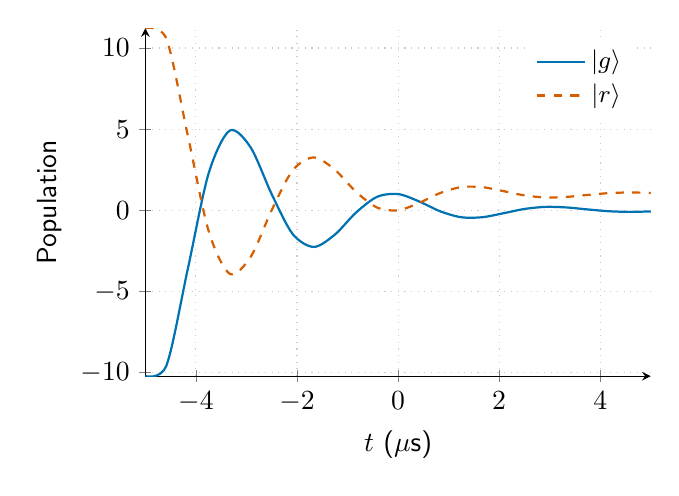
\begin{tikzpicture}
\begin{axis}[
    width=8cm, height=6cm,
    xlabel={$t$ ($\mu$s)}, ylabel={Population},
    legend pos=north east, legend style={font=\small, draw=none},
    tick align=outside, axis lines=left,
    grid=major, grid style={dotted, gray!40},
    font=\sffamily,
]
\addplot[oiBlue, thick, smooth] {exp(-x/2)*cos(deg(2*x))};
\addlegendentry{$|g\rangle$}
\addplot[oiVerm, thick, smooth, dashed] {1 - exp(-x/2)*cos(deg(2*x))};
\addlegendentry{$|r\rangle$}
\end{axis}
\end{tikzpicture}
\end{document}
